\documentclass{article}

% Language setting
% Replace `english' with e.g. `spanish' to change the document language
\usepackage[english]{babel}
\usepackage{appendix}
\usepackage{minted}
\usepackage{tcolorbox}
\usepackage{etoolbox}
\BeforeBeginEnvironment{minted}{\begin{tcolorbox}}
\AfterEndEnvironment{minted}{\end{tcolorbox}}
\usepackage{dirtree}
\usepackage{todonotes}
% Set page size and margins
% Replace `letterpaper' with`a4paper' for UK/EU standard size
\usepackage[letterpaper,top=2cm,bottom=2cm,left=3cm,right=3cm,marginparwidth=1.75cm]{geometry}

% Useful packages
\usepackage{amsmath}
\usepackage{graphicx}
\usepackage[colorlinks=true, allcolors=blue]{hyperref}

\usepackage[normalem]{ulem}
\useunder{\uline}{\ul}{}

\title{Advanced Controls Test Bed \\ User Manual}

\author{
  Gregor P. Henze\textsuperscript{1,2,4}
  \and
  Thibault Marzullo\textsuperscript{1} 
  \and
  Nicholas L. Long\textsuperscript{2} 
  \and
  José A. Leiva Vilaplana\textsuperscript{1,3} 
  \and
  Sourav Dey\textsuperscript{1} 
}


%\author{Thibault Marzullo, Nicholas L. Long, Sourav Dey, José A. Leiva Vilaplana, Gregor P. Henze}

\begin{document}
\maketitle

\textsuperscript{1} University of Colorado Boulder, U.S.A.

\textsuperscript{2} National Renewable Energy Laboratory, Golden (CO), U.S.A.

\textsuperscript{3} Universitat Politècnica de Catalunya, Barcelona, Spain.

\textsuperscript{4} Renewable and Sustainable Energy Institute, Boulder (CO), U.S.A.

\begin{abstract}
The Advanced Controls Test Bed (ACTB) is a building performance simulation test bed designed for developing advanced controllers, such as model predictive control (MPC) or reinforcement learning (RL), for the efficient control of building systems. The ACTB relies on Spawn of EnergyPlus (or Spawn) for high-fidelity models, and on BOPTEST/Alfalfa for simulation management and controller benchmark.
This document describes the prerequisites, installation, and usage of the ACTB from model design to controller evaluation. The user will be capable of generating a high-fidelity Spawn model, designing a simple controller, configuring the simulation and generating results. The manual also presents a practical application, the design and control of a Spawn reference Small Office Building.
\end{abstract}

\section{Introduction}\label{s:intro}

The ACTB is designed to provide a flexible test bed for model designers, control engineers, HVAC manufacturers and researchers to develop advanced control sequences. This guide therefore covers the following topics in distinct sections:
\begin{itemize}
    \item Installing the ACTB and its prerequisites
    \item Designing a Spawn model
    \item Preparing the model for BOPTEST
    \item Loading and simulating a model in the ACTB
    \item Preparing an external controller script
    \item Generating results
    \item Using the OpenAI Gym interface
    \item Using the DO-MPC interface
\end{itemize}

%For clarity, Table TK \todo{reformat table, does not fit BBox} below summarizes terms that are used interchangeably throughout the document.

%\begin{table}[]
%    \centering
%    \begin{tabularx}
%& \textbf{Names} & \textbf{Description} \\    
%Alfalfa & BOPTEST-service & Alfalfa has been partially merged under the BOPTEST-service branch of %the BOPTEST project. The ACTB uses the components of Alfalfa present in the BOPTEST-service branch. %\\
%    \end{tabularx}
%    \caption{Caption}
%    \label{tab:my_labrel}
%\end{table}

\section{Framework}\label{s:framework}

The ACTB's framework is presented in Figure \ref{fig:actb-framework}. The ACTB builds on BOPTEST, a framework for the standardized benchmark of control sequences for building systems. BOPTEST and its underlying Alfalfa components are used as the simulation engine for the ACTB, providing simulation management capabilities and acting as an interface between external controllers and building models. The simulation engine can theoretically\footnote{Currently, the ACTB has only been tested with Modelica-based FMUs.} simulate any model as long as it is packaged in a FMU\footnote{Alfalfa also accepts OpenStudio Workflows (.osw) and EnergyPlus models (.idf) but these features are not yet supported in the ACTB} format.
The controller design is not constrained, the ACTB can read sensors and overwrite controls using the real-world equivalent of software override points as specified by the user. The only constraint is that the data must be exchanged as floating point variables, no other data types are currently supported. The ACTB uses HTTP requests for communicating with the simulation engine, making the framework both operable remotely (e.g. cloud service) and agnostic to the user's programming language. The ACTB and BOPTEST include controller examples both in Python and Julia.
Section \ref{s:dev-spawn} describes the design of a high-fidelity Spawn model, as shown on the top third of Figure \ref{fig:actb-framework}, Section \ref{s:client-api} describes the usage of a general-purpose controller and Section \ref{s:advctrl} introduces the OpenAI Gym and DO-MPC interfaces. 

\begin{figure}
    \centering

    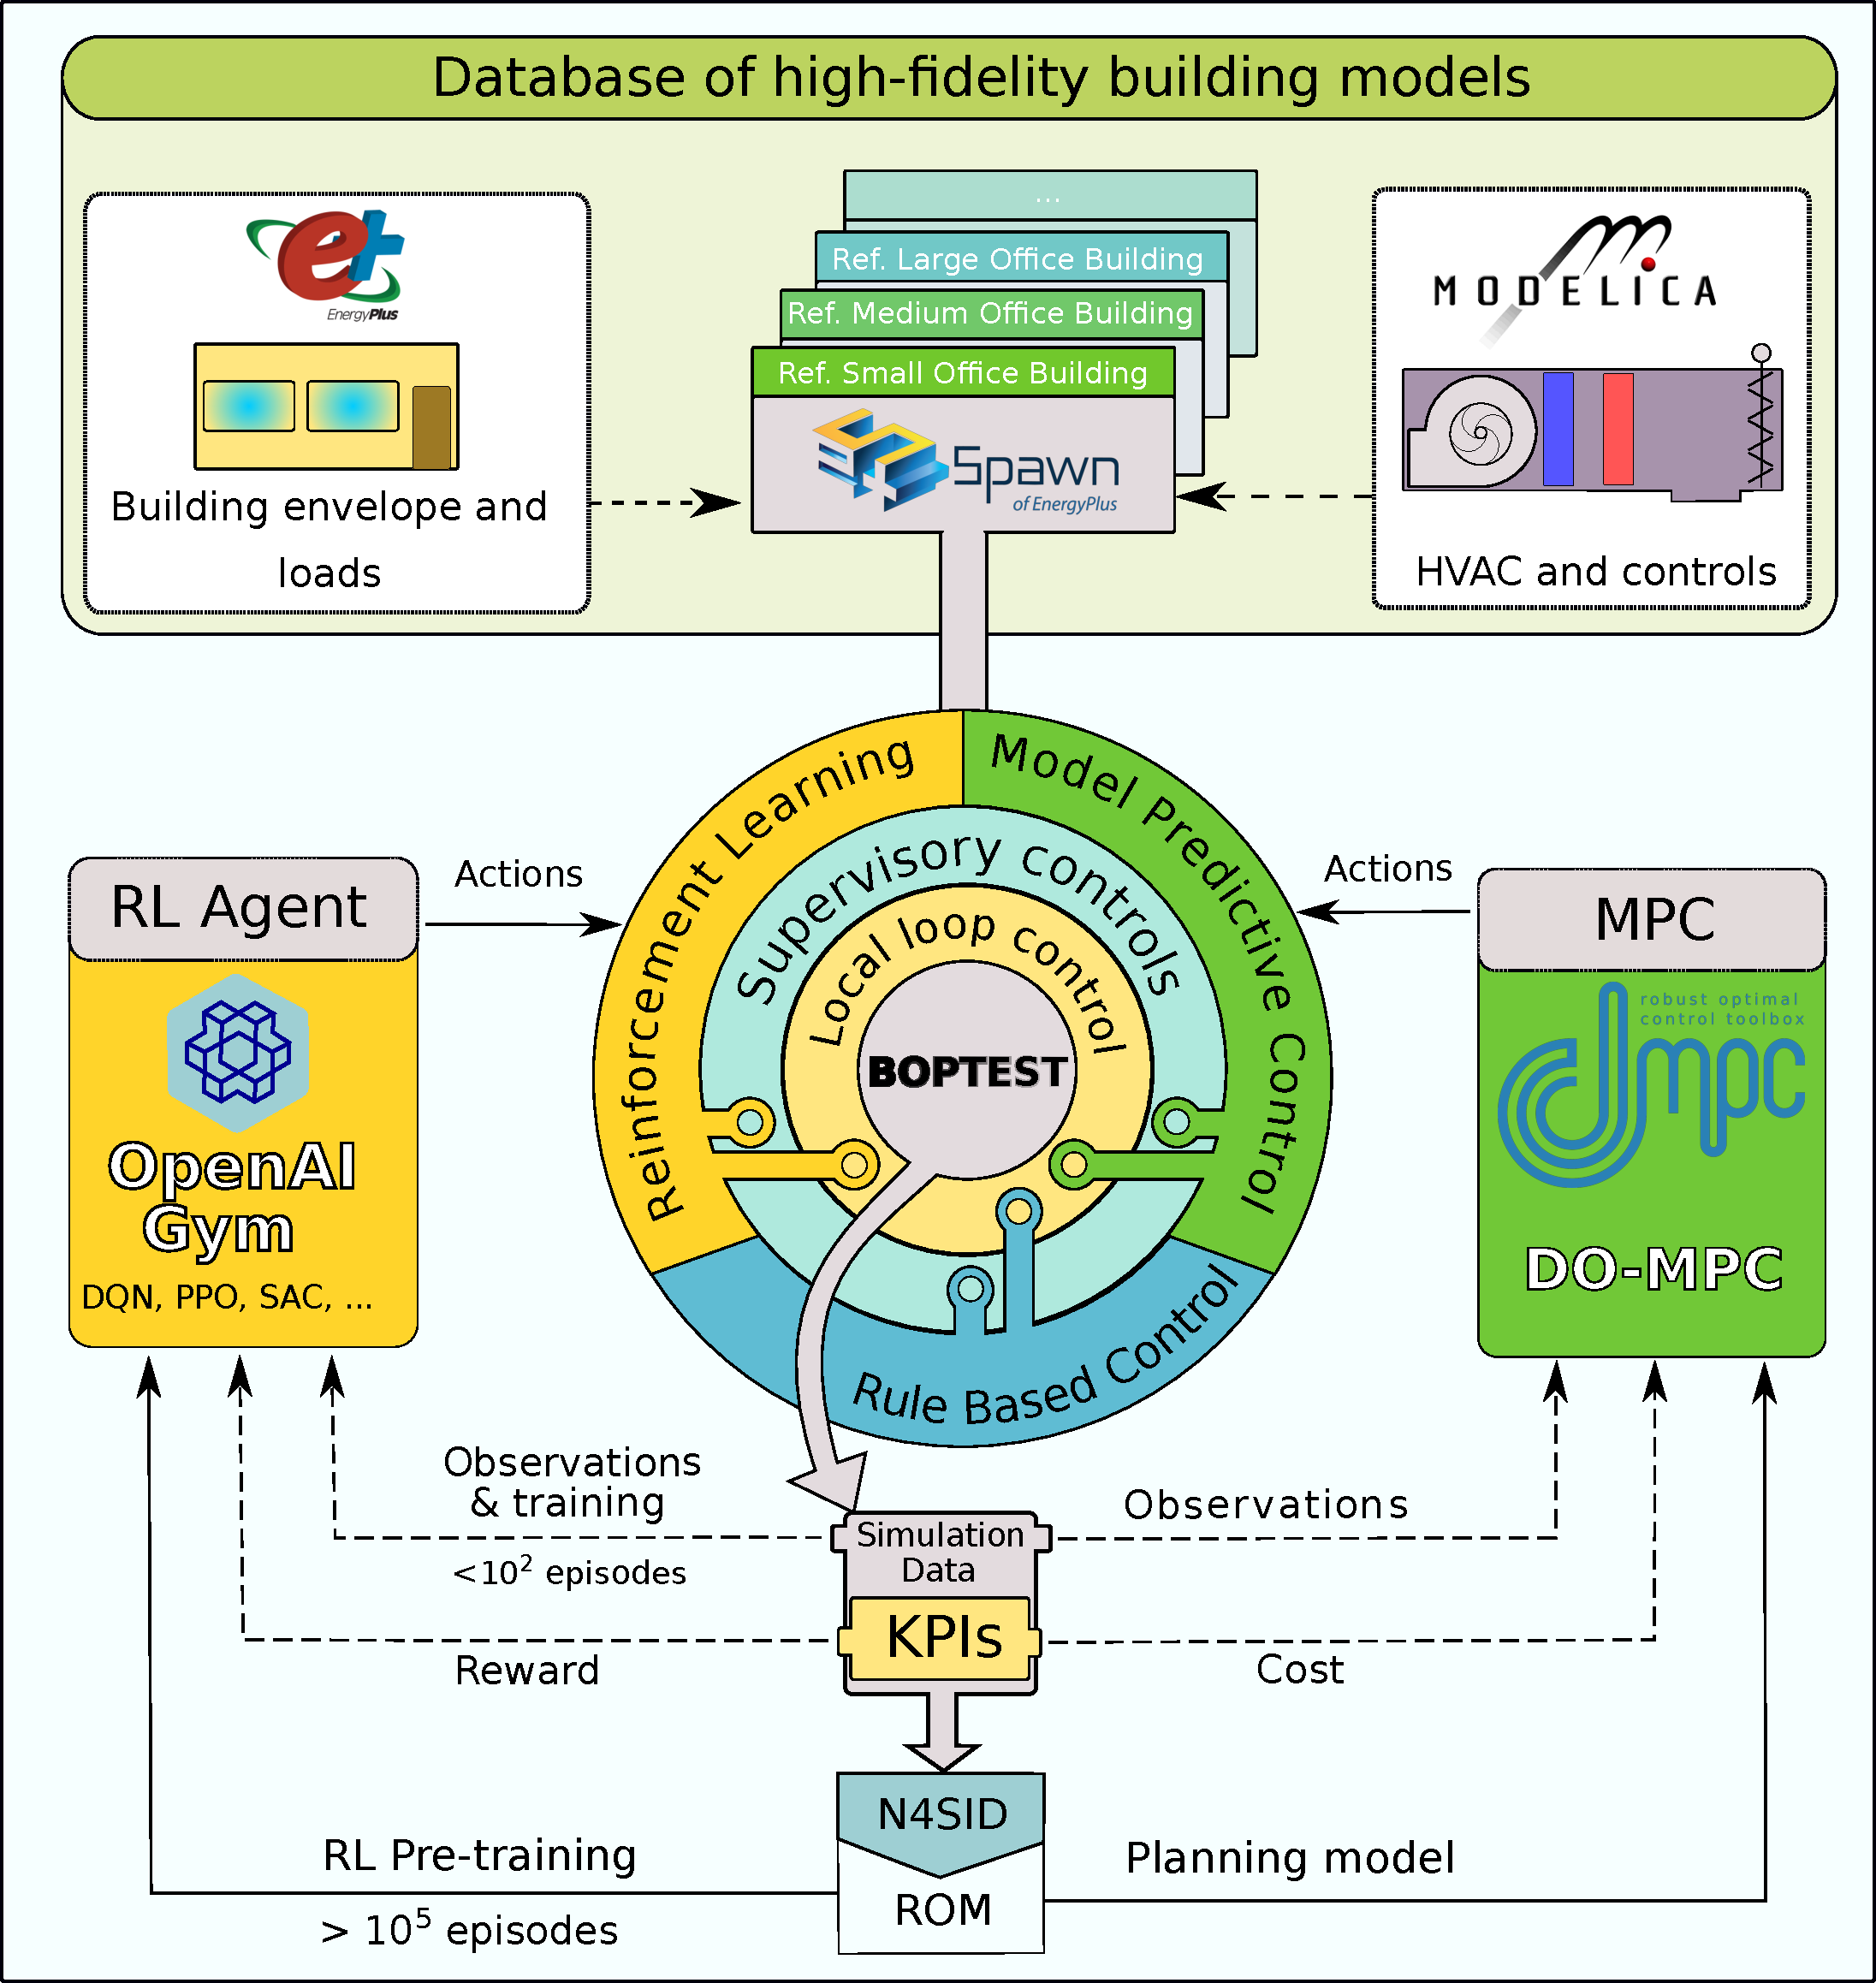
\includegraphics[width=400pt]{Figures/ACTB_v4.pdf}
    \caption{Graphical description of the ACTB framework.}
    \label{fig:actb-framework}
\end{figure}

\section{Installation}\label{s:install}

\subsection{Pre-requisites}\label{s:prereq}

The pre-requisites for installing the ACTB are the following:
\begin{itemize}
    \item A 64-bit UNIX machine;
    \item Python 2.7+, 3.6+ preferred;
    \item Git, \href{https://git-scm.com/}{available here}:
    \item Docker;
\end{itemize}
Optionally, the user might install the following packages:
\begin{itemize}
    \item OpenAI Gym, a machine learning framework \href{https://gym.openai.com/}{available here};
    \item DO-MPC, a robust-MPC framework \href{https://www.do-mpc.com/en/latest/}{available here};
    \item SIPPy, a system identification package \href{https://github.com/CPCLAB-UNIPI/SIPPY}{available here};
    \item A Modelica IDE and simulation engine for model development.\footnote{This manual shows examples using Dassault Systèmes' Dymola 2021.} 
\end{itemize}

\subsection{Installing the ACTB}\label{s:install-actb}

Simply clone the latest version of the ACTB \href{https://github.com/henze-research-group/MODRLC}{from GitHub}.
\begin{minted}{shell-session}
    cd <install_dir>
    git clone https://github.com/henze-research-group/MODRLC
\end{minted}

Run tests to verify that the installation is working correctly:
\begin{minted}{shell-session}
    cd <install_dir>/MODRLC/testing
    python %\todo{cleanup and add the test script}
\end{minted}

If tests do not complete successfully, please make sure that Docker is installed correctly, and that you are using the right version of Python. 

\subsection{Project structure}\label{s:projectstructure}

You will find the following folder tree in the install directory:
\bigskip
\dirtree{%
.1 MODRLC.
.2 boptest\_client.
.2 data.
.2 forecasts.
.2 \textbf{examples}.
.2 kpis.
.2 parsing.
.2 \textbf{template}.
.2 \textbf{testcases}.
.2 testing.
.2 web.
.2 worker.
}
\bigskip
The \verb examples  and \verb testcases  folders contain the provided example controllers and available test cases, respectively. The \verb template  folder contains a Spawn model template. Other folders include BOPTEST resources and utilities (data, forecasts, kpis, parsing, testing) and Alfalfa source-code (web, worker). The user is not required to know or modify any of these files, their usage is not covered in this manual, but more information can be found on \href{https://github.com/ibpsa/project1-boptest}{BOPTEST's} and \href{https://github.com/NREL/alfalfa}{Alfalfa's} web pages. 

\subsection{Quick start}\label{s:quickstart}

This section will demonstrate how to start the ACTB and run a sample simulation of the Reference Small Office Building. The model files are located in the \verb testcases\smallofficechicago  folder and the example simulation script is in the \verb examples\python  folder.
To start the worker, open a terminal session and \verb cd  to the root of your ACTB directory. Then, execute:

\begin{minted}{shell-session}
    docker-compose up web
\end{minted}

When all services have started, \verb cd  to the \verb examples\python  folder of your ACTB install and run the example simulation script\footsnote{On first start, the worker will build all Docker containers, which could take some time.}:

\begin{minted}{shell-session}
    python sim_smalloffice.py
\end{minted}

The script will upload the test case FMU to the worker, initialize the simulation, and run a simple supervisory control loop that simulates a demand-response event.

%\subsection{First use}\label{s:firstuse}

%The ACTB is distributed as a docker container, which needs to be built on first use. This operation will happen once on first launch and subsequently the docker image will be stored on the system.
%To run a sample test case and build the Docker container: 
%\begin{verbatim}
%    cd <install_dir>/MODRLC/
%    sudo make build TESTCASE=<testcase_name>
%\end{verbatim}
%replace \verb <install_dir>  with the path where the ACTB has been installed and \verb <testcase_name>  with the folder name containing the test case you wish to simulate. All test cases are stored in the 

\section{Developing a test case}\label{s:dev-testcase}

This section provides guidance for the design, resource generation and compilation of a Spawn building model, prepared for simulation in the ACTB. It will also cover the usage of MBL's\footsnote{Modelica Buildings Library} \verb signalExchange  blocks to provide sensor and control points that will be used to interface the model to an external controller. 

\subsection{Pre-requisites}\label{s:dev-testcase:prereq}

This section will describe the development of a Spawn building model. The user should therefore:
\begin{itemize}
    \item have good knowledge of the Modelica equation-based language;
    \item have an IDE capable of simulating models from the MBL;
    \item have selected an EnergyPlus building model to enhance;
    \item have installed and tested the ACTB.
\end{itemize}

\subsection{Developing a model}\label{s:dev-spawn}

The ACTB is provided with a sample test case, a \textit{Spawn of EnergyPlus} model. \textit{Spawn} builds on the \textit{EnergyPlusToFMU}  program, which is a utility for packaging an EnergyPlus model into an FMU, or Functional Mock-Up unit\footnote{The Functional Mock-Up unit is a standard format for model exchange and co-simulation built on the FMI standard, \href{https://fmi-standard.org/}{read more about it here}.}. \textit{Spawn} can simulate an EnergyPlus envelope and loads model inside the Modelica environment, using model exchange, allowing the designer to model building systems and their control loops in Modelica. The model can be exported in a portable FMU and then simulated in an environment like the ACTB, where it will use the EnergyPlus simulation engine to provide envelope and load calculations, and the Modelica simulation engine to accurately simulate the desired building systems.

\subsubsection{The building model}

Spawn is an ongoing project, and some features are missing or need revision. The current shortcomings that ACTB developers are aware of are listed below. Issues marked with * are planned to be solved in future Spawn updates.

\begin{itemize}
    \item Spawn becomes unresponsive if the model is simulated beyond Dec. 31st of the simulated year. *
    \item Portable Spawn FMUs do not have a consistent folder structure, the user must post-process the model to ensure directories are correct. *
    \item Spawn thermal zones do not warm-up, the routine is interrupted after the first iteration, before the solution has converged.
    \item Relative paths are changed to absolute paths when specifying model resources for a portable FMU\footnote{this is not strictly a Spawn issue}.
\end{itemize}

Spawn is included as a component of the Modelica Buildings Library v9.0 (MBL). Spawn comes as a two-part component, found under \textit{Buildings/Thermal Zones/EnergyPlus}: a \textit{building} and a series of \textit{thermal zones}. The \textit{building} component shown in Figure \ref{fig:spawn-bldg} is used to specify the following model parameters:
\begin{itemize}
    \item the path to the EnergyPlus building model (.idf),
    \item the path to the weather file (.mos),
    \item the portability of the Spawn model\footnote{the ACTB requires a portable Spawn FMU.},
    \item whether the component also provides a weather bus, from the specified weather file,
    \item the verbosity of the EnergyPlus simulation.
\end{itemize}

\begin{figure}
    \centering
    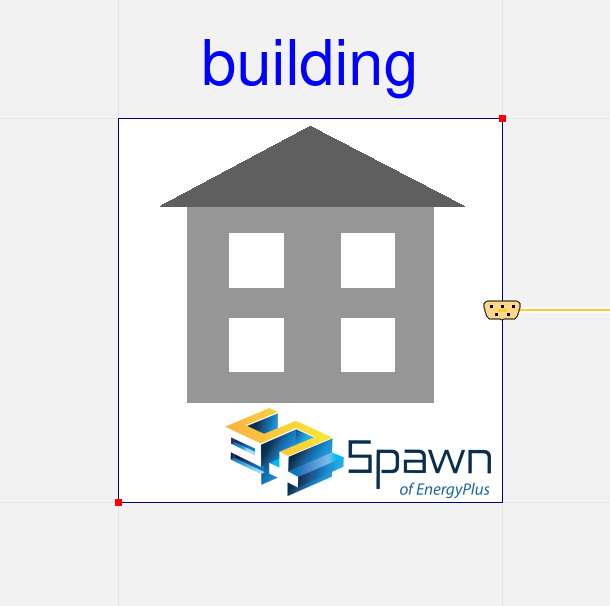
\includegraphics[width=100pt]{Figures/spwnBldg.png}
    \caption{The \textit{building} component.}
    \label{fig:spawn-bldg}
\end{figure}

Figures \ref{fig:spawn-bldg-gen} through \ref{fig:spawn-bldg-adv} show the building component's \textit{General}, \textit{Debug} and \textit{Advanced} tabs respectively. In the General tab, when specifying the paths to the model and weather files, the user should pay close attention to not filling the field with a string, but rather with:
\begin{minted}{modelica}
    Modelica.Utilities.Files.loadResource("path/to/file")
\end{minted}
Where "path/to/file" can be an absolute path or a URI in the form:
\begin{minted}{modelica}
    /absolute/path/to/file
    relative/path/to/file
    modelica://path/within/modelica/libraries
\end{minted}
%\todo{include explanation of how some relative file paths become absolute when compiling into an FMU. Test a URL download from a Docker container on localhost maybe?}

\begin{figure}
    \centering
    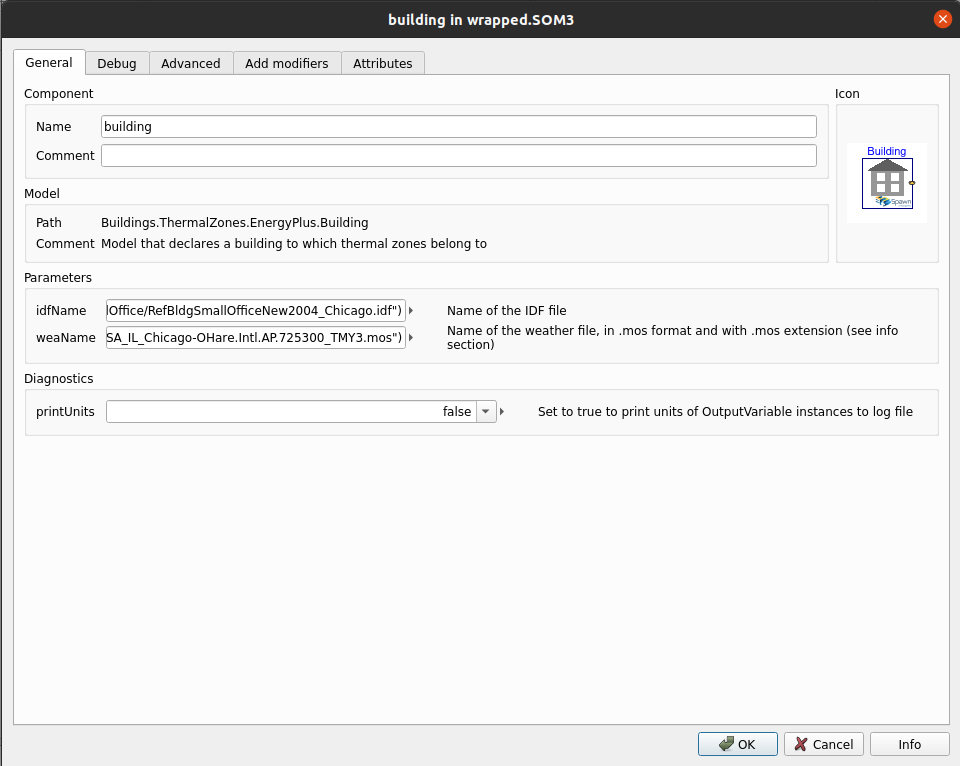
\includegraphics[width=400pt]{Figures/spwn_bldg_general.png}
    \caption{Dymola Graphical User Interface showing the \textit{building}'s "General" tab, where the user must specify the path to the .idf model and the .mos weather file.}
    \label{fig:spawn-bldg-gen}
\end{figure}

\begin{figure}
    \centering
    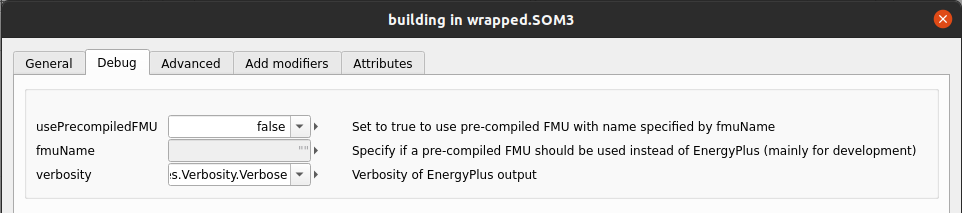
\includegraphics[width=400pt]{Figures/spwn_bldg_debug.png}
    \caption{The \textit{building}'s "Debug" tab.}
    \label{fig:spawn-bldg-deb}
\end{figure}

\begin{figure}
    \centering
    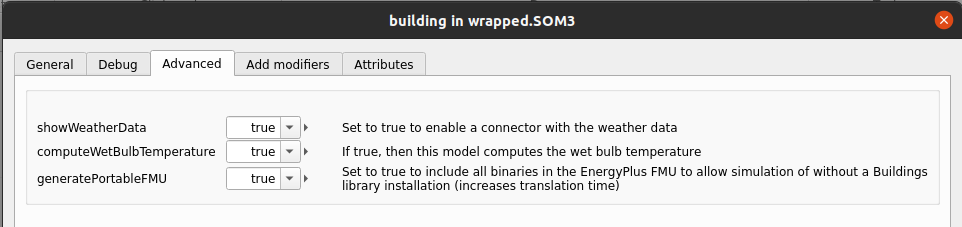
\includegraphics[width=400pt]{Figures/spwn_bldg_advanced.png}
    \caption{The \textit{building}'s "Advanced" tab, where the user can specify if they want to be able to generate a portable FMU or expose a weather bus from the file specified in the "General" tab}
    \label{fig:spawn-bldg-adv}
\end{figure}

After the user has parametrized the \textit{building} component, they can proceed to defining thermal zones. Spawn includes the \textit{ThermalZone} component, which model the zone as a mixing volume with fluid and heat ports that can be connected to the rest of the Modelica model. The user must pay attention to specifying the correct zone name in the \verb zoneName  field. This name is case-sensitive and must match the zone name in the .idf file. The initialization currently has no effect as the building envelope is not warmed-up, as explained above.

\begin{figure}
    \centering
    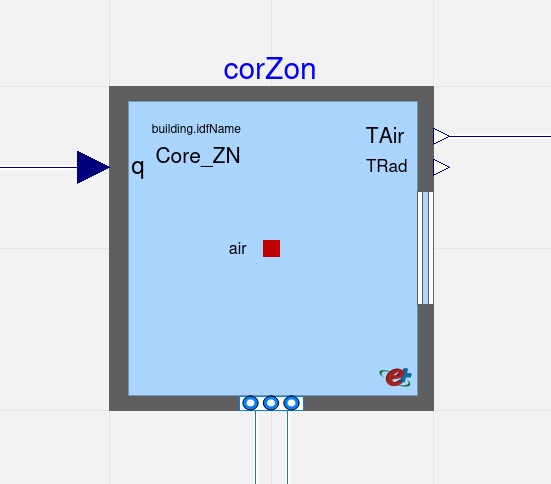
\includegraphics[width=100pt]{Figures/spwn_thrmlzn.png}
    \caption{The \textit{ThermalZone} component}
    \label{fig:spawn-thzn}
\end{figure}

\begin{figure}
    \centering
    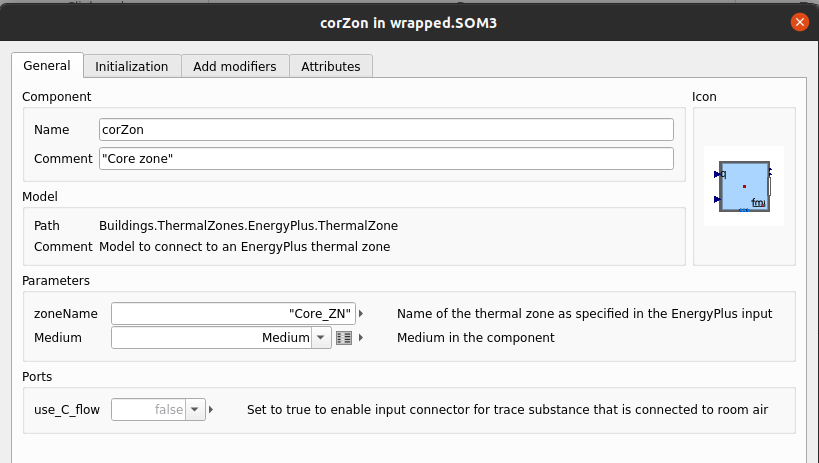
\includegraphics[width=400pt]{Figures/spwn_thrmlzn_general.png}
    \caption{The "General" tab of the \textit{ThermalZone} component, showing the zoneName  field. The user must pay attention to using the same zone names as in the .idf file.}
    \label{fig:spawn-thzn-gen}
\end{figure}

\begin{figure}
    \centering
    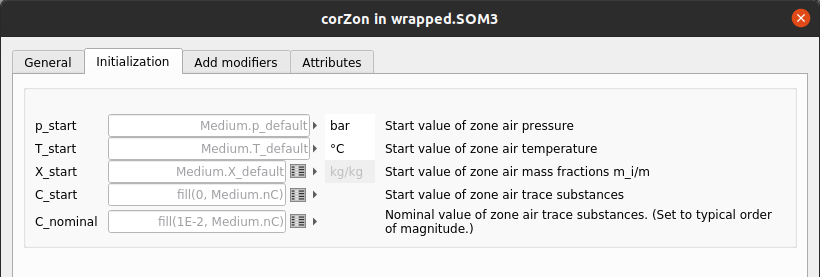
\includegraphics[width=400pt]{Figures/spwn_thrmlzn_advanced.png}
    \caption{The "Advanced" tab of the \textit{ThermalZone} component, showing the zoneName field. While the fluid medium will be initialized to these values, the building envelope is not warmed-up as explained previously, hence the building's thermal mass will drive the building's temperature away from these initial values.}
    \label{fig:spawn-thzn-adv}
\end{figure}

The user can generate as many \verb ThermalZone s as necessary, and it is not required to model all the thermal zones originally present in the .idf.
The \verb ThermalZone s provide a variety of fluid and heat ports, inputs and outputs, and the user is encouraged to familiarize themselves with all the exposed variables and ports in the component's Modelica description. The example provided with the ACTB, for instance, uses the \verb ThermalZone 's heat port, fluid ports, and mean air temperature output. 
With the \verb building  and the \verb ThermalZone  components, the Modelica model can now exchange data with the EnergyPlus simulation engine.

Apart from \verb signalExchange  blocks, presented in the next section, the rest of the model is left to the user's imagination, as it will not differ from another standard Modelica model. Users are strongly encouraged to visit \href{https://www.modelica.org/libraries}{the Modelica libraries webpage} to learn more about the possibilities offered by Modelica modeling.

\subsubsection{signalExchange read and write blocks}

In order to read and write to the Spawn model, the ACTB leverages signalExchange blocks. These components come in two flavors: the read and the write block. While both blocks are placed on a control line or on a sensor output, they differ in usage and functionality.
\textit{read} blocks, presented in Figure \ref{fig:sigex-readwrite} , are used to expose sensor readings. Figure \ref{fig:sigex-read} shows how a \textit{read} block is parametrized. The user should first select the "KPIs" drop-down menu, and specify whether the value that this block reads is used for KPI calculation or not. For some KPIs, the "zone" field should comport a string indicating which zone is being reported on. The "y" field specifies the output's unit and limits.

Similarly, the \textit{write} block shown in Figure \ref{fig:sigex-readwrite} is parametrized as shown in Figure \ref{fig:sigex-write}. The user must only specify the unit and limits of the "u" input, which will be used to override the signal the block is placed onto. The \textit{read} blocks include a hidden property, the \textbf{\_activate} flag, which is used to choose whether the block overrides the signal or lets it pass through. 

\begin{figure}
    \centering
    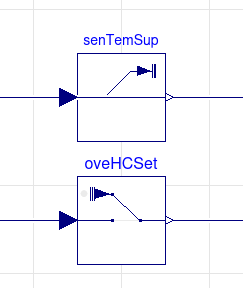
\includegraphics[width=100pt]{Figures/readwrite.png}
    \caption{The \textit{read} (top) and \textit{write} (bottom) blocks}
    \label{fig:sigex-readwrite}
\end{figure}

\begin{figure}
    \centering
    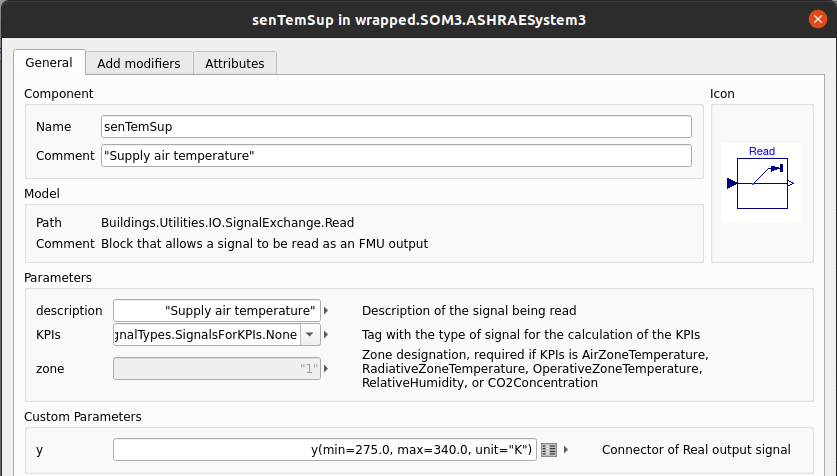
\includegraphics[width=400pt]{Figures/readblock.png}
    \caption{The \textit{read} block's parameters}
    \label{fig:sigex-read}
\end{figure}

\begin{figure}
    \centering
    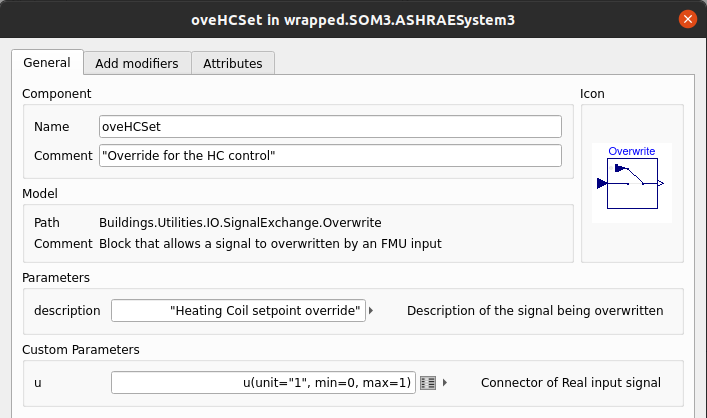
\includegraphics[width=400pt]{Figures/write_block.png}
    \caption{The \textit{write} block's parameters}
    \label{fig:sigex-write}
\end{figure}

The user must pay attention to including the minimum and maximum values and the unit for each \textit{read} and \textit{write} block. In both blocks, the user should add a custom parameter that defines the upper and lower bounds of the input or output, and the unit. For \textit{write} blocks, the user should include:
\begin{minted}{modelica}
    u(min=<min_value>, max=<max_value>, unit="<unit>")
\end{minted}

The full declaration for a sample \textit{write} block is
\begin{minted}{modelica}
    Buildings.Utilities.IO.SignalExchange.Overwrite oveCooSetpoint(u(
            unit="K",
            min=0,
            max=310), description="Cooling setpoint override")
\end{minted}

For \textit{read} blocks, the user should include:

\begin{minted}{modelica}
    y(min=<min_value>, max=<max_value>, unit="<unit>")
\end{minted}

The full declaration of a sample \textit{read} block becomes:

\begin{minted}{modelica}
    Buildings.Utilities.IO.SignalExchange.Read senOcc(y(
    min=0.0, 
    max=10.0, 
    unit="1"), description="occupancy sensor",
    KPIs=Buildings.Utilities.IO.SignalExchange.SignalTypes.SignalsForKPIs.None)
\end{minted}

\subsection{Exporting the model and resources}\label{s:dev-fmu}

Once the Modelica model has been designed and saved as a .mo file, the user should create a new folder in the "testcases" folder. The folder name should be in lower case characters, with no spaces. In that folder, the user should include model documentation in the "doc" folder and model files and resources in the "models" folder. Resources should go in a folder named "Resources" (case-sensitive). The user can use the template provided in the "template" folder, it contains model and resources templates, as well as the directory structure.
After the directories have been generated, the user should see the following folder structure:

\dirtree{%
.1 ACTB\_root. 
.2 testcases. 
.3 mymodelname. 
.4 config.py. 
.4 benchmark.py. 
.4 library\_versions.json. 
.4 docs. 
.5 model\_documentation.pdf. 
.4 models. 
.5 mymodel.mo. 
.5 Resources. 
.6 electricity\_prices\_dynamic.csv. 
.6 emission\_factors.csv. 
.6 \dots . 
}
In order to export the model, the user must update the following files:
\begin{itemize}
    \item config.py: update the model step, forecast horizon, and energy pricing scenario
    \item models\textbackslash compile\_fmu.py: update \verb mopath  and \verb modelpath .
    \item models\textbackslash library\_versions.json: update the hash of the MBL commit, if needed.
    \item models\textbackslash resources\textbackslash *: verify that all data has been generated correctly by the data\_manager.py script.
\end{itemize}

Once the test case directory is ready, and all files have been updated to correspond to the current model, the model should be compiled into an FMU. 
To do that, \verb cd  into the \verb <ACTB_root_dir>\testing\  directory and run the following command:
\begin{verbatim}
    sudo make compile_testcase_model TESTCASE=<testcase_folder_name>
\end{verbatim}

If all resources are available, the script should complete and generate two files: \verb wrapped.mo  and \verb wrapped.fmu  , which are respectively the model wrapper that maps FMU inputs and outputs, and the self-contained FMU that will be used in the simulation manager. You can now move or copy the \verb wrapped.fmu  archive to a more convenient location, and later upload it to the ACTB.

\subsection{Additional design considerations}

TK include Spawn considerations, file paths explanation for FMU export, notes on Windows, etc.

\section{Using the ACTB}\label{s:actb-usage}

This section of the user manual provides guidance for interfacing an external controller to a model that has already been prepared and compiled into an FMU. 

\subsection{Startup}

In order to interact with the ACTB, its Docker container must be active, and running. First, start a terminal window\footnote{you may need elevated privileges for some commands, a common sign of insufficient privileges is a refused access or connection. Simply add "sudo" before the commands} and \verb cd  to the root folder of the ACTB. To verify which containers are currently active, use:

\begin{verbatim}
    docker container ls
\end{verbatim}

If you already have active Docker containers, they will be listed there. The command to start the ACTB through Alfalfa depends on the number of simulation workers that the user needs. By using the \verb docker-compose  commands described below, the user will be launching BOPTEST-service, or the Alfalfa-based simulation manager version of BOPTEST. \footsnote{This is the intended usage of the ACTB, however users can decide to bypass Alfalfa and use only the BOPTEST portion. Users are invited to refer to BOPTEST's user guide available \href{https://github.com/ibpsa/project1-boptest}{here} in that case.}


\bigskip    

\textit{\textbf{Single simulation worker:}}

To start a single simulation worker, \verb cd  to the ACTB root folder and use:

\begin{verbatim}
    docker-compose up web
\end{verbatim}

This is the terminal output that you should see if the service has started correctly: 

\begin{minted}{shell-session}
    user@machine:~$  sudo docker-compose up web
    Starting modrlc_redis_1 ... done
    Starting modrlc_minio_1 ... done
    Starting modrlc_goaws_1 ... done
    Starting modrlc_mongo_1 ... done
    Starting modrlc_mc_1    ... done
    Starting modrlc_worker_1 ... done
    Starting modrlc_web_1    ... done
    Attaching to modrlc_web_1
\end{minted}

Please note that the container name prefix, here \verb modrlc  , is automatically selected to match that of the parent folder. The rest of the names are formatted in a standard way:  \textit{folder\_service\_ID}

To stop the Docker containers, first stop the process with Ctrl+C and use:
\begin{verbatim}
    docker-compose down 
\end{verbatim}

You will see the Docker containers stopping:

\begin{minted}{shell-session}
    user@machine:~$  sudo docker-compose down
    Stopping modrlc_worker_1 ... done
    Stopping modrlc_redis_1  ... done
    Stopping modrlc_mongo_1  ... done
    Stopping modrlc_goaws_1  ... done
    Stopping modrlc_minio_1  ... done
    Removing modrlc_web_1    ... done
    Removing modrlc_worker_1 ... done
    Removing modrlc_mc_1     ... done
    Removing modrlc_redis_1  ... done
    Removing modrlc_mongo_1  ... done
    Removing modrlc_goaws_1  ... done
    Removing modrlc_minio_1  ... done
    Removing network modrlc_default
\end{minted}

\bigskip    

\textit{\textbf{Multiple simulation workers:}}

To start multiple simulation workers, \verb cd  to the ACTB root folder and use:

\begin{minted}{python}
    docker-compose up --scale worker=<number_of_workers>
\end{minted}
where \verb <number_of_workers>  is an integer number representing the number of simulation workers that are desired.  

TK: Ask Nick about the fact that messages are queued, and delays are long, so the single HTTP queue seems to be slowing down the process quite a bit. Do several web containers solve the issue?

If the command is successful, you should see the Docker containers starting. In the following example, 7 workers are launched:

\begin{minted}{shell-session}
    user@machine:~$  sudo docker-compose up --scale worker=7
    Creating network "modrlc_default" with the default driver
    Creating modrlc_minio_1 ... done
    Creating modrlc_mongo_1 ... done
    Creating modrlc_goaws_1 ... done
    Creating modrlc_redis_1 ... done
    Creating modrlc_mc_1    ... done
    Creating modrlc_worker_1 ... done
    Creating modrlc_worker_2 ... done
    Creating modrlc_worker_3 ... done
    Creating modrlc_worker_4 ... done
    Creating modrlc_worker_5 ... done
    Creating modrlc_worker_6 ... done
    Creating modrlc_worker_7 ... done
    Creating modrlc_web_1    ... done
    Attaching to modrlc_minio_1, modrlc_mongo_1, modrlc_goaws_1, modrlc_redis_1, 
    modrlc_mc_1, modrlc_worker_2, modrlc_worker_4, modrlc_worker_3,
    modrlc_worker_7, modrlc_worker_1, modrlc_worker_6, modrlc_worker_5, modrlc_web_1
\end{minted}

Please note that unlike the command for launching a single worker, stopping the Alfalfa stack will automatically stop the Docker containers that have been started. By doing Ctrl+C, the following output confirms that all containers were stopped:

\begin{minted}{shell-session}
    Gracefully stopping... (press Ctrl+C again to force)
    Stopping modrlc_web_1    ... done
    Stopping modrlc_worker_6 ... done
    Stopping modrlc_worker_5 ... done
    Stopping modrlc_worker_4 ... done
    Stopping modrlc_worker_7 ... done
    Stopping modrlc_worker_2 ... done
    Stopping modrlc_worker_3 ... done
    Stopping modrlc_worker_1 ... done
    Stopping modrlc_redis_1  ... done
    Stopping modrlc_mongo_1  ... done
    Stopping modrlc_goaws_1  ... done
    Stopping modrlc_minio_1  ... done
\end{minted}

While the ACTB relies on its Alfalfa component to upload new models on demand, it is technically possible to build a dedicated BOPTEST Docker container that includes one or several building models. This usage is not the main purpose of the BOPTEST framework and will not be covered in this user guide, but some information is presented to the user who wishes to use the ACTB differently.

\subsection{Client API}\label{s:client-api}

While the ACTB is running, the user can interact with the simulation worker by sending RESTful requests or by using the Alfalfa client API. The client API is a more user-friendly method for interacting with the simulation worker. The available RESTful requests are reported\footnote{reproduced from BOPTEST's user guide \href{https://github.com/ibpsa/project1-boptest}{here}} in Table \ref{tab:restful}. For example, in Python, a user who needs to fetch the model name can use\footnote{assuming that the \textit{requests}  Python package has been installed. See \href{https://pypi.org/project/requests/}{the project's PyPi webpage}}:

\begin{minted}{python}
    import requests
    url = 'http://127.0.0.1:5000'
    name = requests.get('{0}/name'.format(url)).json()
\end{minted}

The ACTBleverages Alfalfa's Python API\footsnote{See \href{https://pypi.org/project/alfalfa-client/}{the Alfalfa-Client's Pypi entry}} which can be installed either manually or with pip:

\begin{minted}{shell-session}
    pip install alfalfa-client
\end{minted}

After installing the client, the user can use it in their code by importing the client and historian if needed:

\begin{minted}{python}
    import alfalfa_client.alfalfa_client as ac
    import alfalfa_client.historian as ah

    client = ac.AlfalfaClient
    historian = ah.Historian
\end{minted}

The user can then use the methods reported in Table \ref{tab:alfalfaapi} to control the simulation, read sensor data and write commands to/from the simulated building systems. More methods are available, but are not needed by the user directly. Please refer to Alfalfa's \href{https://github.com/NREL/alfalfa}{GitHub webpage} for more information on the Alfalfa client.

\renewcommand{\arraystretch}{1.5}
\begin{table}\tiny
\resizebox{\textwidth}{!}{%
\begin{tabular}{p{150pt}|p{150pt}}
\hline
\midrule
Request                                                                                                                                                & Description                                                                                                                                                                  \\
\hline
\multicolumn{2}{c}{PUT}                                                                                                                                                                                                                                                                                                               \\
\hline
PUT initialize with arguments start\_time=, warmup\_time=                                                                                              & Initialize simulation to a start time using a warmup period in seconds                                                                                                       \\
\hline
PUT step with argument step=\textless{}value\textgreater{}                                                                                             & Set communication step in seconds.                                                                                                                                           \\
\hline
PUT results with arguments point\_name=, start\_time=, final\_time=                                                                                    & Receive test result data for the given point name between the start and final time in seconds.                                                                               \\
\hline
PUT forecast\_parameters with arguments horizon=, interval=                                                                                            & Set boundary condition forecast parameters in seconds.                                                                                                                       \\
\hline
PUT scenario with optional arguments electricity\_price=, time\_period=. See README in /testcases for options and test case documentation for details. & Set test scenario. Setting the argument time\_period performs an initialization with predefined start time and warmup period and will only simulate for predefined duration. \\

\hline
\multicolumn{2}{c}{GET}                                                                                                                                                                                                                                                                                                               \\
\hline
GET step                                                                                                                                               & Receive communication step in seconds.                                                                                                                                       \\
\hline
GET measurements                                                                                                                                       & Receive sensor signal point names (y) and metadata.                                                                                                                          \\
\hline
GET inputs                                                                                                                                             & Receive control signal point names (u) and metadata.                                                                                                                         \\
\hline
GET kpi                                                                                                                                                & Receive test KPIs.                                                                                                                                                           \\
\hline
GET name                                                                                                                                               & Receive test case name.                                                                                                                                                      \\
\hline
GET forecast                                                                                                                                           & Receive boundary condition forecast from current communication step.                                                                                                         \\
\hline
GET forecast\_parameters                                                                                                                               & Receive boundary condition forecast parameters in seconds.                                                                                                                   \\
\hline
GET scenario                                                                                                                                           & Receive current test scenario.                                                                                                                                               \\
\hline
\multicolumn{2}{c}{POST}                                                                                                                                                                                                                                                                                                              \\
\hline
POST advance with json data "\{:\}"                                                                                                                    & Advance simulation with control input and receive measurements.              \bottomrule                                                                                               
\end{tabular}}
\caption{List of RESTful requests and their usage}
\label{tab:restful}
\end{table}

\begin{table}\tiny
\resizebox{\textwidth}{!}{%
\begin{tabular}{l|l}
\textbf{Method}         & \textbf{Description}                                 \\ 
\hline
submit(path)            & Upload a model found in path. Returns a site object. \\
start(site, kwargs)     & Start a site and initialize the simulation           \\
setInputs(site, inputs) & Set the control vector of a site                     \\
advance({[}sites{]})    & Step the simulation of a list of sites               \\
outputs(site)           & Retrieve results from the last step                  \\
stop(site)              & Stop a site                                         
\end{tabular}%
}
\caption{List of useful methods for interacting with the Alfalfa API}
\label{tab:alfalfaapi}
\end{table}


\subsection{Interfacing an external clock and controller}\label{s:controllers}

The user can define both an "internal" controller, built into the Spawn model, and an external controller that will read sensor measurements and override one or several control variables. The control variables and sensors are defined in the Spawn model and can be retrieved using the Alfalfa client API described in Section \ref{s:client-api}.

The typical usage of the external controller is as follows:
\begin{enumerate}
    \item \textbf{Initialize the simulation worker:} set up the communication parameters, and set simulation parameters such as the step in seconds, and the simulation start and end time in seconds. Initialize a historian if needed.
    \item \textbf{Retrieve test case information:} retrieve useful information from the model, such as the available control points or sensor points.
    \item \textbf{Initialize the control vector:} the \textbf{u} control vector can be any combination of available inputs, or can be left empty. Please refer to Section TK \ref{}.
    \item \textbf{Step the simulation:} at each step the simulation returns the sensor readings, which can be used to update the control vector. It is possible to retrieve the last set of KPIs at any time in the process.
    \item \textbf{Update the control vector:} this can be any function that yields a formatted \textbf{u} control vector.
    \item \textbf{Retrieve results:} at the end of a simulation, the results are stored until the Docker container is reset, along with the KPIs calculated over the entire simulation run. 
\end{enumerate}

A simple controller that uses the Alfalfa client API will look as follows: 

\begin{minted}{python}
    import os
    from alfalfa_client import AlfalfaClient, Historian
    
    end_time = 365 * 24 * 3600
    alfalfa = AlfalfaClient(url='http://localhost')
    file = os.path.join(os.path.dirname(__file__), 'files', 'wrapped.fmu') 
    site = alfalfa.submit(file)
    alfalfa.start(
        site,
        external_clock="true",
        end_datetime=end_time
    )
    for i in range(steps):
        y = 
        u = process_controls(y)
        alfalfa.setInputs(site, u)
    
\end{minted}

Below, an example using HTTP requests as shown in Table \ref{tab:restful}:

\begin{minted}{python}
    import requests, json, collections, os
    url = 'http://0.0.0.0:5000'
    length = 1 * 24 * 3600
    step = 300
    simStartTime = 186*24*3600
    warmupPeriod = 30 * 24 * 3600

    # GET TEST INFORMATION
    # --------------------

    name = requests.get('{0}/name'.format(url)).json()
    inputs = requests.get('{0}/inputs'.format(url)).json()
    measurements = requests.get('{0}/measurements'.format(url)).json()
    step_def = requests.get('{0}/step'.format(url)).json()

    # RUN TEST CASE
    # -------------

    res = requests.put('{0}/initialize'.format(url), 
                        data={
                            'start_time': simStartTime, 
                            'warmup_period': warmupPeriod})
    res = requests.put('{0}/step'.format(url), data={'step': step})
    u = initializeControls()  
    for i in range(int(length / step)):
        y = requests.post('{0}/advance'.format(url), data=u).json()

        u = rulebased.compute(y)

    # POST PROCESS RESULTS
    # --------------------

    res = requests.get('{0}/results'.format(url)).json()
    kpi = requests.get('{0}/kpi'.format(url)).json()
\end{minted}

For details on interfacing an OpenAI Gym agent or DO-MPC, please refer to Section \ref{s:advctrl}.

\subsection{Additional simulation considerations}

Users should be aware of the following limitations, and should regularly check if a new ACTB release is available:

\begin{itemize}
    \item 
\end{itemize}

\section{Advanced controller interfaces}\label{s:advctrl}

The ACTB includes interfaces to two popular machine learning and MPC toolboxes: the OpenAI Gym framework and DO-MPC. Both interfaces are based in Python, and this manual assumes that the user has already installed and tested the packages. 

\subsection{OpenAI Gym}\label{s:openai}

A custom Gym environment wrapper is included with the ACTB, which acts as an interface between Gym and the RESTful API.
First, the user should instantiate the custom Gym environment and provide the following information:
\begin{itemize}
	\item \textbf{Time variables}: length, start time and time step of the simulation, in seconds.
	\item \textbf{Actions}: the control points, as displayed when requesting the available model inputs.
	\item \textbf{Reward function}: The custom Gym environment uses BOPTEST built-in KPIs to calculate the reward function. The user can specify the KPIs to return for computing the reward at each control step, as well as the weighing (linear and exponential) of the objective. The weighing consists of one linear and exponential hyper-parameter. The type of KPI objectives could be any subset of the KPIs provided by BOPTEST. These could be energy, thermal discomfort, indoor air quality discomfort, CO\textsubscript{2} emissions and operational costs. The user can specify to return the KPIs from all zones or only a subset with the \verb kpi_zones  argument, and the rewards are summed over all the zones. 
    \item \textbf{Observation states}: There are two types of observation states that needs to be specified - one is the set of observation states from the building sensors while the other one is external weather variables and the associated forecast\footsnote{currently, the weather forecast is assumed perfect.}. These two type of variables are concatenated and are returned as full observation states to the RL controller agent.
\end{itemize}


Below, an example of building environment that interfaces a RL agent to the included Reference Small Office Building test case:

\begin{figure}[H]
\singlespacing
\begin{minted}{python}
episode_length = 24 * 3600    # Simulate for a day
step = 300                    # Setting Step size in seconds 
start_time = 3*24*3600        # Start from the third day of the year
kpi_zones = ["1"]             # Select the zones for the reward function 

actions = ['oveHeaSet1_u']

building_obs = ['senTRoom1_y','senHou_y']
forecast_obs = {'TDryBul': [4], 'TWetBul': [0], 'HGloHor': [0]}

''' Final observations are the combined 'building_obs' and 'forecast_obs' '''

# Customize the reward objective -- uses BOPTEST KPIs
KPI_rewards  = { "ener_tot": {"hyper": -20, "power": 2},
                 "tdis_tot": {"hyper": -50, "power": 1},
                 "idis_tot": {"hyper": 0,   "power": 1},
                 "cost_tot": {"hyper": 0,   "power": 1},
                 "emis_tot": {"hyper": 0,   "power": 1} }
# --------------------

env = BoptestGymEnv( max_episode_length=episode_length,
                     Ts                = step,
                     actions           = actions,
                     building_obs      = building_obs,
                     forecast_obs      = forecast_obs,
                     lower_obs_bounds  = [273,  0, 273, 273, 0,   0],
                     upper_obs_bounds  = [330, 24, 330, 330, 4, 700],
                     kpi_zones         = kpi_zones,
                     KPI_rewards       = KPI_rewards,
                     start_time        = start_time)
\end{minted}
\caption{Setting up a RL problem}
\label{fig:openai-env-ex}
\doublespacing
\end{figure}

The user can control the simulation as described in Section \ref{s:client-api}, with the addition of the following methods for the custom environment:

\begin{itemize}
\item \textit{step([actions])}: returns a tuple composed of the current state, rewards, and additional custom information that can be defined in TK ADD SCRIPT NAME. The \textit{step()} function takes a list of actions as an input.
\item \textit{reset()}: resets all the building states to the initial start time. 
\item \textit{get\textunderscore building\textunderscore states()}: returns the current building states at as a dictionary. 
\item \textit{get\textunderscore weather\textunderscore forecast()}: returns the current weather and its forecast. 
\item \textit{get\textunderscore KPIs()}: returns the sum of all KPIs %\todo{Sourav, is it the sum of all zones for a type of KPI or the sum of all KPIs on all zones?}. 

\end{itemize}

\subsection{DO-MPC}

\section{Additional features}

\subsection{N4SID model reduction}

\appendix
\appendixpage
\addappheadtotoc

\section{DOE Reference Small Office Building}

\subsection{Design of a Spawn model for the ACTB}

\subsection{Design of a Python controller interface}

\subsection{Simulation in the ACTB and results}

\section{DOE Reference Medium Office Building}

\subsection{Design of a Spawn model for the ACTB}

\subsection{Design of a Python controller interface}

\subsection{Simulation in the ACTB and results}

\bibliographystyle{alpha}
\bibliography{sample}

\end{document}